\chapter{Izračun}


V tem poglavju bom s primerom dokazal, da program računa parametre pretočne hidroelektrarne pravilno. Za dokaz bom uporabil namišljen primer trapezno oblikovane struge vodotoka prikazane na sliki~\ref{fig:izracun_trapeznaStruga} z Manningovim koeficientom hrapavosti 0,3 in z 1\% naklonom struge. Rezultate ročnega izračuna bom primerjal z rezultati ki jih izračuna program po trapezni in numerični metodi opisani v poglavju~\ref{sec:pretok_prav_trapez}  oz.~\ref{sec:pretokNumericnaMetoda}. Vse mere na spodnji sliki so v metrih.



\begin{figure}[ht!]
	\begin{centering}
		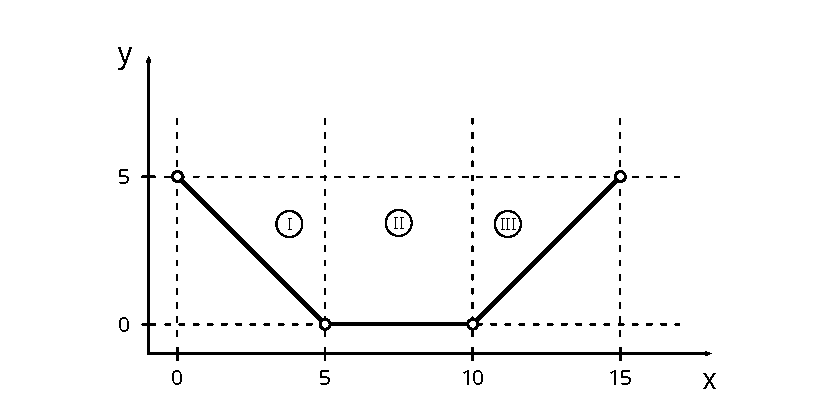
\includegraphics[width=\textwidth]{slike/izracuni/trapeznaStruga.pdf}		
		\caption{Shema struge izbranega vodotoka}\label{fig:izracun_trapeznaStruga}
	\end{centering}
\end{figure}

\section{Ročni izračun parametrov hidroelektrarne}

\begin{enumerate}[I.]
	
	\item Odsek
	
	\begin{ceqn}
		\begin{align}
			S_I&=\dfrac{5 * 5}{2} = 12,5~m^2\\
			P_I&=\sqrt{5^2 + 5^2} = 7,07~m\\
			Q_I&=\dfrac{\sqrt{0,01}}{0,03} * \dfrac{12,5^{5/3}}{7,07^{2/3}} = 60,9~m^3/s
		\end{align}
	\end{ceqn}
		
	\item Odsek
	
	\begin{ceqn}
		\begin{align}
			S_{II}&=5*5 = 25 ~m^2\\
			P_{II}&=5 = 5~m\\
			Q_{II}&=\dfrac{\sqrt{0,01}}{0,03} * \dfrac{25^{5/3}}{5^{2/3}} = 243,7~m^3/s
		\end{align}
	\end{ceqn}
	
	\item Odsek
	\begin{ceqn}
		\begin{align}
		S_{III}&=S_{I} = 12,5~m^2\\
		P_{III}&=S_{I} = 7,07~m\\
		Q_{III}&=Q_{III} = 60,9~m^3/s
		\end{align}
	\end{ceqn}
	
\end{enumerate}

Skupni pretok:

\begin{ceqn}
 \begin{align}
Q_{s} = Q_{I} + Q_{II} + Q_{III} = 60,9 + 243,7 + 60,9 = 365,5~m^3/s
 \end{align}
 \end{ceqn}




\section{Izračun parametrov hidroelektrarne s programom}

\subsection{Izračun parametrov s trapezno metodo}
%TODO:


\subsection{Izračun parametrov z numerično metodo}

S pomočjo uporabniškega vmesnika v koordinatni sistem vnašamo serijo točk, s katerimi modeliramo robove izbrane struge. V tabeli na levi strani diagrama, za vsak odsek med dvema točkama dodajamo Manningove koeficiente hrapavosti $ng$ in naklone struge na sliki označene s $\varphi$. V našem primeru so vrednosti koeficientov za vse odseke rečne struge enake.

\begin{figure}[ht!]
	\begin{centering}
		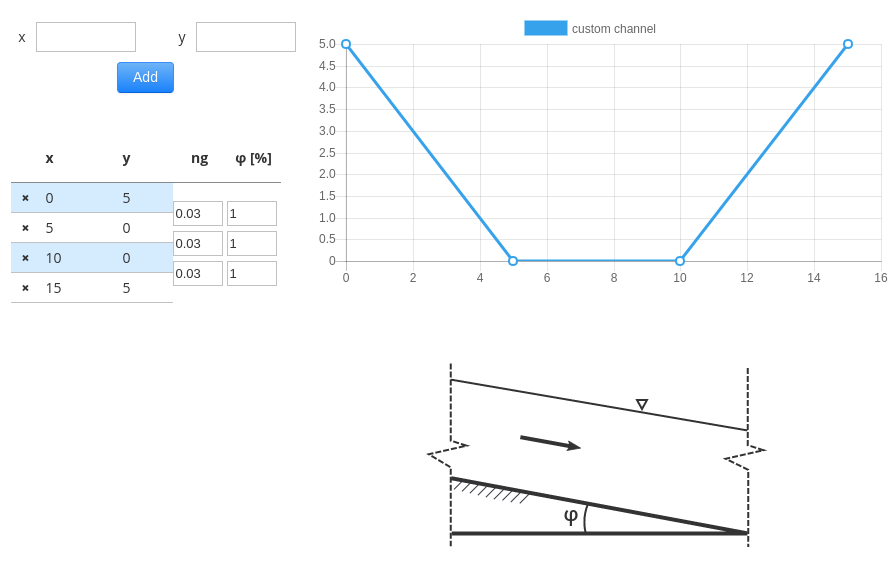
\includegraphics[width=\textwidth]{slike/izracuni/modeliranjeStruge.png}		
		\caption{Vnos podatkov v program}\label{fig:modeliranjeStruge}
	\end{centering}
\end{figure}

% H forces image to stand here on this place -> pushes text below
\begin{figure}[H]
	\begin{centering}
		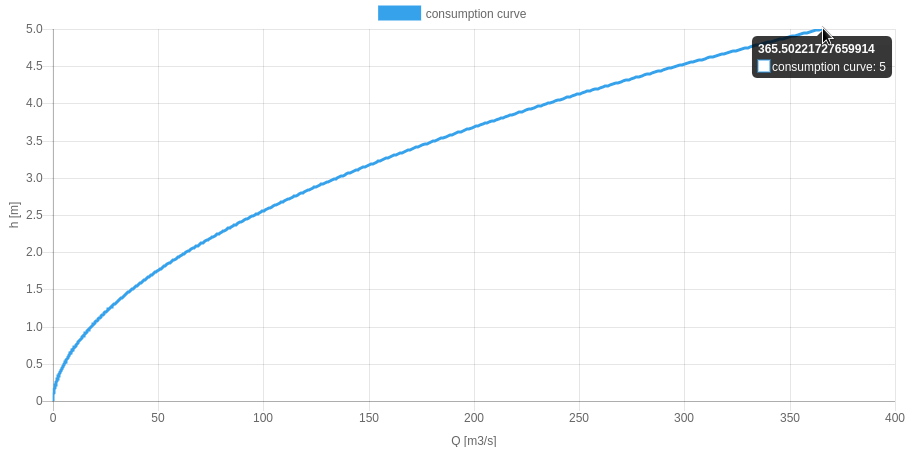
\includegraphics[width=\textwidth]{slike/izracuni/consumptionCurve.png}		
		\caption{Graf konsumpcijske krivulje}\label{fig:custom_konsumpcijskaKrivulja}
	\end{centering}
\end{figure}


Z grafa konsumpcijske krivulje pri višini $h = 5m$ lahko preberemo da se rezultat numerične metode ujema z rezultatom ki smo ga izračunali ročno.

